% !TEX encoding = UTF-8
% !TEX TS-program = pdflatex
% !TEX root = ../tesi.tex

%**************************************************************
\chapter{Obiettivi dello stage}
\label{cap:obiettivi}
%**************************************************************

% SSO IMAGE SOURCE https://www.getkisi.com/courses/sso-guide

\section{Vantaggi aziendali}
    \textbf{Zextras} ospita stage di questa tipologia da ormai diversi anni nonostante sia un'attività che richiede un quantità di tempo e impegno non indifferente poiché, costringe l'azienda a sottrarre risorse dai progetti e dalle attività in corso che, molto spesso, sono vincolate da scadenze. Tuttavia i vantaggi portati da uno strumento come lo stage sono molteplici. Per prima cosa l'azienda ha la possibilità di condurre dei progetti di ricerca che molto spesso coinvolgono l'utilizzo di nuove tecnologie, senza essere costretta a rallentare lo sviluppo dei prodotti ordinari e soprattutto riducendo il rischio di investire troppe risorse in progetti che potenzialmente potrebbero non proseguire. \\
    Alternativamente ha la possibilità affidare ad uno studente lo sviluppo di un prodotto non particolarmente complesso al fine di inserirlo gradualmente nel mondo del lavoro (o nell'organico aziendale) e, allo stesso tempo, far risparmiare tempo al resto del \textit{team}.
    Un altro aspetto interessante dal punto di vista aziendale è il poter entrare in contatto con studenti che, seppur privi di esperienza lavorativa, sono spesso in grado di proporre soluzioni alternative e creative a problemi comuni. I vantaggi elencati si sono effettivamente concretizzati nel tempo, infatti negli utlimi anni il \textit{team} di sviluppo ha integrato nel suo organico alcuni studenti che, una volta completato lo stage, sono rimasti a contribuire alle sfide tecnologiche che l'azienda affronta giornalmente. \\
    Ciò significa che uno stage ben organizzato e seguito si rivela essere un vero e proprio investimento, non solo per l'azienda che lo ospita, la quale beneficerà degli \textit{output} di questa attività, ma anche per la crescita degli studenti, i quali diventeranno le figure professionali che nel futuro faranno parte dell'intera industria la quale, soprattutto negli ultimi anni, necessita di molte risorse vista la sua dinamicità.

\newpage

\section{Presentazione del progetto}\label{sec:progetto}
    Questo progetto nasce dall'esigenza di rendere disponibile un nuovo sistema di autenticazione per la \textit{webmail} di \gls{zcsg}, in grado di fornire il giusto connubio tra sicurezza e facilità d'uso. \textbf{Zextras} utilizza molti strumenti e servizi al suo interno, sia per lo sviluppo sia per l'amministrazione. Questi utilizzano \gls{okta} per la gestione dell'autenticazione, ciò significa che è sufficiente effettuare una sola autenticazione con il proprio account \gls{okta} per poter poi accedere a tutti i servizi ad esso collegati. \\
    Questa tipologia di autenticazione si chiama \gls{sso} e consiste nell'utilizzo di una singola credenziale che permette di accedere a più servizi. \\
    \gls{zcsg} era l'unico serivizio, uno dei più utilizzati in azienda, che non beneficiava di questa tecnica di autenticazione. Per questo motivo \textbf{Zextras} prende la decisione di esplorare la possibilità di sviluppare un sistema personalizzato che, oltre all'autenticazione base, avesse le seguenti caratteristiche:
    \begin{itemize}
        %\setlength\itemsep{0em}
        \item quando un utente che possiede un \textit{account} su \gls{okta} ma non su \gls{zcsg}, accede per la prima volta su quest'ultima, viene creato un nuovo account su \gls{zcsg}, associato a quello di \gls{okta};
        \item importazione su \gls{zcsg} delle informazioni utente presenti su \gls{okta};
        \item sincronizzazione dei gruppi di \gls{okta} ai quali un utente appartiene, con liste di distribuzione e classi di servizio di \gls{zcsg}.
    \end{itemize}
    Il fine di questo progetto era quello di uniformare il metodo di autenticazione di \gls{zcsg} rispetto a tutti gli servizi utilizzati dall'azienda e soprattutto avere un sistema personalizzato e configurabile che permette di automatizzare alcune operazioni ripetitive e dispendiose in termini di tempo.
    Per poter proporre una soluzione conforme alle esigenze emerse, ho dovuto per prima cosa condurre uno studio e un'analisi dei protocolli di autenticazione presenti sul mercato. La seconda parte invece consisteva nella progettazione e implementazione del sistema, utilizzando il protocollo ritenuto più idoneo.
    
    \begin{figure}[ht]
        \centering
        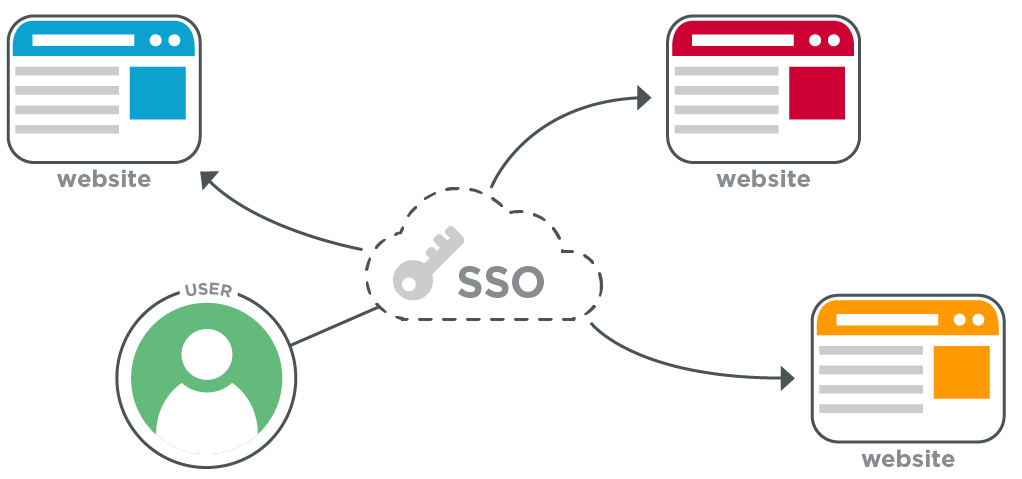
\includegraphics[width=0.75\textwidth]{immagini/sso.png}
        \caption{\textit{Single Sign-On}}
        \textbf{Fonte}:
        \href{https://developer.fourth.com/en-gb/docs/single-sign-saml}{developer.fourth.com}
        \label{fig: Single Sign-On}
    \end{figure}


    \subsection{Analisi stato dell'arte protocolli di autenticazione}\label{sec:att_analisi}
    %Descrizione dell'attività di analisi e di studio dei protocolli di autenticazione che ho dovuto condurre come prima attività durante lo stage.
    La prima attività che ho dovuto svolgere era la ricerca e lo studio dei protocolli di autenticazione più diffusi e utilizzati sul mercato. L'azienda conosceva già alcuni di questi, ma voleva avere un'analisi approfondita e degli esempi del loro utilizzo. Inoltre poteva rivelarsi una valida occasione per scoprire nuovi possibili protocolli adatti all'implementazione del sistema di autenticazione. \\
    L'azienda ha quindi richiesto di redigere un documento che riportasse tutti i risultati delle mie ricerche, in particolare l'analisi dei pro e dei contro di ciascun protocollo e la sua applicabilità al problema da risolvere.

    \subsection{Progettazione di un sistema di autenticazione personalizzato}
        In seguito all'analisi svolta, il secondo obiettivo dello stage era la progettazione, seguita dall'implementazione, di un sistema di autenticazione per \gls{zcsg} utilizzando il protocollo scelto da me, guidato dal \textit{team} di sviluppo. Il sistema di autenticazione doveva essere in grado di:
        \begin{itemize}
            \setlength\itemsep{0em}
            \item utilizzare \gls{okta} come \gls{idpg};
            \item supportare altri \gls{idpg} che utilizzato lo stesso protocollo;
            \item supportare \gls{zcsg} tramite il \gls{ssog} di \gls{okta} rendendo opzionale l'accesso tramite \textit{email} e \textit{password};
            \item garantire sicurezza.
        \end{itemize}
    \begin{figure}[ht]
        %\setlength{\textfloatsep}{1pt}
        %\setlength{\belowcaptionskip}{1pt}
        \centering
        
\includegraphics[width=0.75\textwidth]{immagini/rd.jpg}
        \caption{\textit{Research \& Development}}
        \textbf{Fonte}:
        \href{https://youteam.io/blog/research-and-development-the-fourth-pillar-of-software-development/}{youteam.io}
        \label{fig: Research & Development}
    \end{figure}

\section{Vincoli}
    \subsection{Vincoli metodologici}
        Per lo svolgimento dell'attività di stage è stato deciso, in comune accordo con il \textit{tutor}, che il modo più efficace per portarla a termine, fosse lavorando presso la sede aziendale. La prima motivazione deriva dalla metodologia di sviluppo adottata, descritta nella sezione \secref{sec:met_svilpuppo}, la quale è fortemente incentrata sulla comunicazione e sul confronto frequente con tutti i membri nel \textit{team}. Inoltre, poiché sarei stato affiancato da alcuni \textit{senior developer} si trattava di un'ottima occasione per apprendere il più possibile da professionisti nel settore.
        Oltre agli incontri di allineamento giornalieri, il \textit{Project Manager} ha stabilito che ci sarebbero stati degli incontri formali, insieme al \textit{tutor} aziendale, per fare il punto della situazione. Nella fase conclusiva del progetto era inoltre prevista una \textit{\gls{demog}} a cui avrebbero presenziato altre figure aziendali appartententi a diversi reparti.
        %\begin{itemize}
        %    \item il \textit{CEO} dell'azienda;
        %    \item il \textit{Project Manager};
        %    \item il responsabile tecnico dell'azienda;
        %    \item il \textit{team} di sviluppo con il \textit{tutor} aziendale;
        %    \item il responsabile di un altro \textit{team};
        %\end{itemize}
        La presenza di figure appartenti a diversi settori e \textit{team} sarebbe state utile a discutere il prodotto sviluppato, sia dal punto di vista funzionale sia da quello infrastrutturale. Inoltre, ricevere un \textit{feedback} da punti di vista diversi è certamente utile per il miglioramento dell'applicazione nel suo insieme.
        
        \begin{figure}[ht]
            \centering
            
\includegraphics[width=0.9\textwidth]{immagini/team.jpg}
            \caption{\textit{Teamwork}}
            \textbf{Fonte}:
            \href{https://www.sandler.com/blog/6-benefits-of-teamwork-in-the-workplace/}{sandler.com}
            \label{fig: Teamwork}
        \end{figure}
\newpage
    \subsection{Vincoli temporali}\label{sec:vincoli_tempo}
    L'attività di stage prevista aveva una durata di 304 ore, da svolgere nell'arco di due mesi, suddivise in 8 settimane della durata di circa 40 ore ciascuna. L'orario di lavoro accordato con l'azienda era dal Lunedì al Venerdì dalle ore 9.00 alle 18.00. \\
    Prima dell'inizio dello stage ho pianificato, insieme al \textit{tutor}, le attività per ciascuna settimana di lavoro, facendone una stima orario per il loro completamento. Sin dal primo giorno io e il \textit{tutor} aziendale abbiamo rispettato il piano di lavoro stabilito. Tuttavia, in seguito all'attività di analisi svolta, come descritto nella sezione \secref{sec:att_analisi}, abbiamo dovuto dedicare più tempo per ottenere un prototipo base funzionante, poiché non era ancora chiaro come utilizzare il protocollo di autenticazione scelto. Nonostante un rallentamento a metà percorso, il resto dello stage ha avuto un andamento lineare che mi ha permesso di terminare il lavoro senza fretta. 
    
    \begin{figure}[ht]
        \centering
        
\includegraphics[width=1\textwidth]{immagini/plan.png}
        \caption{\textit{Planning}}
        \textbf{Fonte}:
        \href{https://www.sysaid.com/blog/entry/8-tips-on-how-to-plan-for-configuration-management-part-1}{sysaid.com}
        \label{fig: Planning}
    \end{figure}
    
    \subsection{Vincoli tecnologici}
    Le tecnologie e i linguaggi utilizzati duarante questo progetto fanno parte dello \textit{stack} tecnologico dell'azienda e sono le seguenti:
    \begin{itemize}
        \item \textbf{Java}: essendo il linguaggio con cui è scritto \gls{zcsg}, ne consegue che tutta la tecnologia di \textbf{Zextras} si sia adeguata, compreso il mio progetto;
        \item \textbf{Git}: sistema di versionamento, come descritto nella sezione \secref{sec:configurazione};
        \item \textbf{Docker}: è una tecnologia che permette di creare, rilasciare ed eseguire delle applicazioni utilizzando un \gls{containerg}. In questo modo l'ambiente racchiuso nel \gls{containerg} potrà essere eseguito, tramite \textit{docker}, su macchine diverse che solitamente hanno diverse configurazioni. Questo comportamente è simile alla virtualizzazione e permette di rendere gli ambienti di esecuzione solidi e deterministici. In particolare l'azienda lo utilizza per creare delle istanze di \gls{zcsg} utilizzate come ambienti di test in fase di sviluppo. La gestione dei \gls{containerg} sono gestiti tramite un servizio di nome \textbf{\textit{Portainer}}\footnote{https://www.portainer.io/}.
    \end{itemize}

    \begin{figure}[ht]
        \centering
        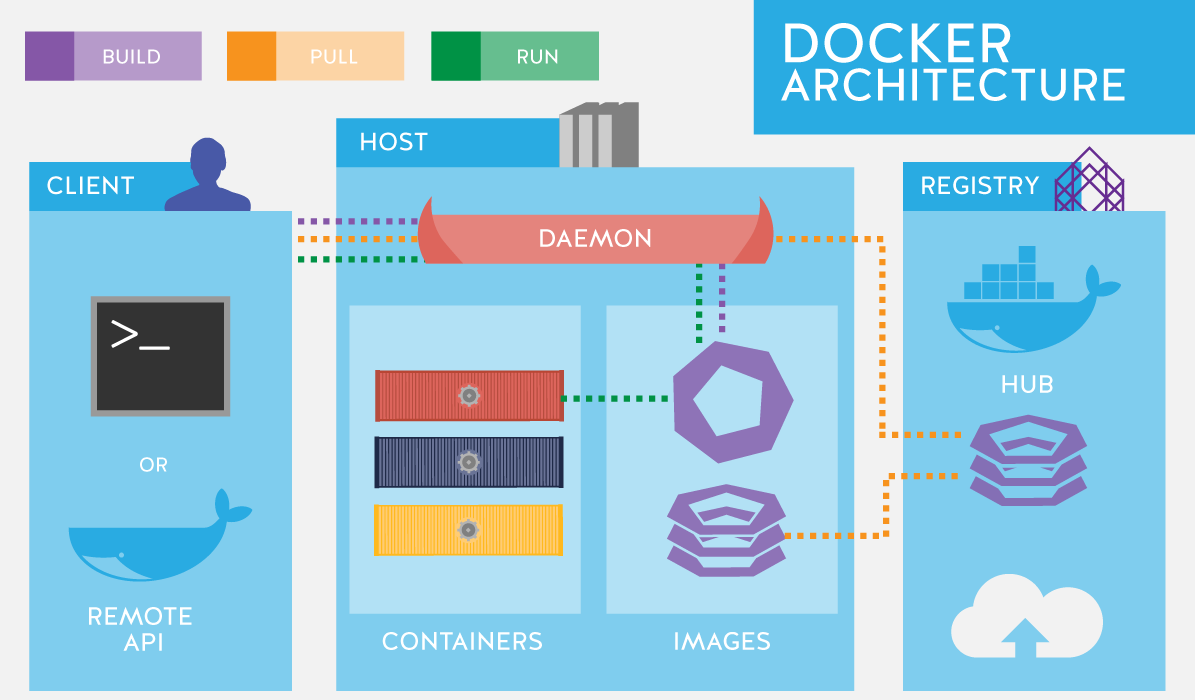
\includegraphics[width=1\textwidth]{immagini/docker.png}
        \caption{\textit{Docker workflow}}
        \textbf{Fonte}:
        \href{https://nordicapis.com/api-driven-devops-spotlight-on-docker/}{nordicapis.com}
        \label{fig: Docker workflow}
    \end{figure}

\section{Aspettative aziendali}\label{sec:aspettative_aziendali}
    %Descrizione degli output che l'azienda si aspettava da questo stage
    Al termine delle 304 ore previste per il completamento dello stage, l'azienda si aspettava di avere almeno l'autenticazione base funzionante che facesse uso del protocollo scelto, in modo da autenticare gli utenti su \gls{zcsg} tramite l'\gls{idpg} \gls{okta}. Come già descritto in precedenza però, la parte interessante di questo progetto era l'aggiunta di alcune funzionalità personalizzate ad un sistema di autenticazione standard. Per questo motivo dopo aver concluso l'attività di ricerca sui protocolli, descritta nel paragrafo \secref{sec:att_analisi}, ho discusso, insieme al \textit{team} e al \textit{Project Manager}, i requsiti specifici da implementare. Ciò è stato utile perché al momento della stesura del piano di lavoro, alcuni di essi non potevano essermi chiari a causa della mancanza di contesto riguardante l'ambiente \gls{zcsg}. Gli obiettivi stabiliti erano suddivisi in due gruppi. In ordine di priorità: \textbf{obbligatori} e \textbf{desiderabili}.
    \paragraph{Obiettivi obbligatori}
    \begin{itemize}
        \item Analisi stato dell'arte dei protocolli di autenticazione più diffusi;
        \item Implemenazione di un sistema di autenticazione per \gls{zcsg} tramite il protocollo scelto;
    \end{itemize}
    \paragraph{Obiettivi desiderabili}
    \begin{itemize}
        \item \textit{\gls{prov}};
        \item Importazione dei dati dell'utente di \gls{okta} su \gls{zcsg};
        \item Flusso di autenticazione a partire sia dall'\gls{idpg} sia da \gls{zcsg};
        \item Controllo della \gls{cosg} di \gls{zcsg} tramite l'\gls{idpg};
        \item Gestione delle \gls{distlistg} di \gls{zcsg} tramite l'\gls{idpg};
        \item Autenticazione a due fattori;
        \item Integrazione con \textit{WebAuthn}\footnote{\url{https://www.w3.org/TR/webauthn-2/}}
    \end{itemize}

\section{Aspettative personali}\label{sec:aspettative_personali}
Nel corso della laurea triennale ho sempre avuto idea di ciò che volessi fare del punto di vista professionale una volta finito gli studi. Tuttavia, prima di specializzarmi in un determinato ambito, ho deciso di esplorare altre realtà sfruttando l'opportunità di svolgere un'attività stage. Ciò che mi interessava quindi, era osservare in prima persona il modo di lavorare di professionisti, l'utilizzo di tecnologie (sia conosciute in ambito accademico sia per me nuove) a livello professionale e apprendere il più possibile sul mondo del lavoro. Inoltre avevo intezione di trovare un progetto di stage che potesse portare del valore concreto all'azienda e soprattutto avere la possibilità di completarlo nell'arco dei due mesi disponibili, invece di lavorare su prototipi usa e getta.
Per poter avere un'idea dell'offerta dell'industria informatica attuale, ho partecipato all'evento \textit{Stage-IT} \footnote{\url{http://informatica.math.unipd.it/laurea/stageit.html}} organizzato dell'Università degli studi di Padova, pensato per mettere in contatto gli studenti con la realtà lavorativa. Durante l'evento ho sostenuto diversi colloqui con aziende che spesso proponevano dei progetti incentrati sull'esplorare una nuova tecnologia ed eventualmente sviluppare un prototipo. Poiché, come già accennato, il mio obiettivo era quello di portare a termine un prodotto finito e utilizzabile, ho continuato la mia ricerca anche dopo lo svolgersi dell'evento. Ho contattato altre aziende e sostenuto altri colloqui finché non ho trovato \textbf{Zextras}, che mi ha convinto fin da subito con il progetto proposto e con l'ambiente lavorativo presentato. Quindi i miei obiettivi da raggiungere con un progetto di stage erano:
\begin{itemize}
    \item lavorare ad un progetto per tutto il suo ciclo di sviluppo. In particolare, partire dalla fase iniziale di ricerca, passare alla fase di progettazione, implementare la soluzione proposta, collaudarlo e vederlo in funzione;
    \item osservare e provare l'utilizzo di linguaggi a me noti in ambito professionale;
    \item esplorare una realtà aziendale che proponesse un metodo di lavoro interessante e significativo anche in altri ambiti dello sviluppo \textit{software};
    \item lavorare ad un progetto \gls{opensg}.
\end{itemize}

    %\begin{figure}[ht]
    %    \centering
    %    
\includegraphics[width=1\textwidth]{immagini/learning.jpeg}
    %    \caption{\textit{Learning}}
    %    \textbf{Fonte}:
    %    \href{https://elearningindustry.com/6-elearning-strategies-develop-deeper-learning-skills}{elearningindustry.com}
    %    \label{fig: Learning}
    %\end{figure}